\section{The Ubhatob­yañ­janaka}
\label{ubhato}
In the \textit{Theravāda} \textit{Vinaya} \textit{Khandhaka} 1 we find the following passage:\footnote{\textit{Khandhaka} 1 \textit{Pabbajjā} PTS vol 1 page 89, translation by Ajahn Brahmali.}

\begin{quote}
\textit{Tena kho pana samayena aññataro ubhatobyañjanako bhikkhūsu pabbajito hoti. So karotipi kārāpetipi. Bhagavato etamatthaṁ ārocesuṁ. Ubhatobyañjanako, bhikkhave, anupasampanno na upasampādetabbo, upasampanno nāsetabboti.}
\end{quote}

\begin{quote}
At one time an \textit{ubhatob­yañ­janaka} had gone forth as a monk. He had sex and made others have it. They told the Buddha and he said, ``An \textit{ubhatob­yañ­janaka} should not be given the full ordination. If it has been given, he should be expelled.''
\end{quote}

Just like with the \textit{paṇḍaka}, the \textit{ubhatob­yañ­janaka} in this passage is already ordained at the time of this incident and in a similar way we can deduce that the rule itself is limited to \textit{upasampadā} (full ordination) while novice ordination is allowed. The commentarial texts again mention that both are prohibited. And just like with the \textit{paṇḍaka} we would expect the subject of the story to be expelled on the grounds of breaking the first rule against intercourse, but instead not only he but also all others like him are expelled. Again, there seems to be a prejudiced perception of these individuals as possessing an inherent flaw that makes them unable to keep their precepts.

For the term \textit{ubhatob­yañ­janaka}\footnote{\textit{Ubhato} meaning `in both ways, on both sides' and \textit{byañjana} or \textit{vyañjana} means `sign or mark'.} we have less material to go on than for the term \textit{paṇḍaka}. They are only briefly mentioned in the Chinese \textit{Vinayas} as those with two roots/faculties (二根) who are not allowed to ordain, but without any further explanation. The Therāvada \textit{Vinaya} merely states that this person ``acted and was acted upon''. 

The commentarial literature is slightly more forthcoming but no less confusing as to the meaning of the word. The \textit{Samantapāsādikā}\footnote{\textit{Samantapādādikā}, vol. 3, para. 116. Translation by Ajahn Brahmali.} states:\footnote{Note that the word \textit{liṅga} is not used here. Instead the word \textit{nimitta} is used to denote `characteristic of sex/gender'.}

\begin{quote}
\textit{Ubhatobyañjanako bhikkhaveti itthinimittuppādanakammato ca purisanimittuppādanakammato ca ubhato byañjanamassa atthīti ubhatobyañjanako.Karotīti purisanimittena itthīsu methunavītikkamaṁ karoti. Kārāpetīti paraṁ samādapetvā attano itthinimitte kārāpeti, so duvidho hoti – itthiubhatobyañjanako, purisaubhatobyañjanakoti.Tattha itthiubhatobyañjanakassa itthinimittaṁ pākaṭaṁ hoti, purisanimittaṁ paṭicchannaṁ. Purisaubhatobyañjanakassa purisanimittaṁ pākaṭaṁ, itthinimittaṁ paṭicchannaṁ. Itthiubhatobyañjanakassa itthīsu purisattaṁ karontassa itthinimittaṁ paṭicchannaṁ hoti, purisanimittaṁ pākaṭaṁ hoti. Purisaubhatobyañjanakassa purisānaṁ itthibhāvaṁ upagacchantassa purisanimittaṁ paṭicchannaṁ hoti, itthinimittaṁ pākaṭaṁ hoti. Itthiubhatobyañjanako sayañca gabbhaṁ gaṇhāti, parañca gaṇhāpeti. Purisaubhatobyañjanako pana sayaṁ na gaṇhāti, paraṁ gaṇhāpetīti, idametesaṁ nānākaraṇaṁ.}

\textit{Kurundiyaṁ pana vuttaṁ--``yadi paṭisandhiyaṁ purisaliṅgaṁ pavatte itthiliṅgaṁ nibbattati, yadi paṭisandhiyaṁ itthiliṅgaṁ pavatte purisaliṅgaṁ nibbattatī''ti. Tattha vicāraṇakkamo vitthārato aṭṭhasāliniyā dhammasaṅgahaṭṭhakathāya veditabbo. Imassa pana duvidhassāpi ubhatobyañjanakassa neva pabbajjā atthi, na upasampadāti idamidha veditabbaṁ.}
\end{quote}

\begin{quote}
The \textit{ubhatob­yañ­janaka} means: Because of \textit{kamma} giving rise to female characteristics and \textit{kamma} giving rise to male characteristics, there is for them the characteristics of both. With the male characteristic they act to transgress through sexual intercourse with women. Having encouraged another, they cause action in their own female characteristic. 

They are twofold: the female \textit{ubhatob­yañ­janaka} and the male \textit{ubhatob­yañ­janaka}. In regard to this, the female characteristic of the female \textit{ubhatob­yañ­janaka} is apparent, but the male characteristic is hidden. The male characteristic of the male \textit{ubhatob­yañ­janaka} is apparent, but the female characteristic is hidden. 

While the female \textit{ubhatob­yañ­janaka} is acting with manliness among women, the female characteristic is hidden, whereas the male characteristic is apparent. 
When the male \textit{ubhatob­yañ­janaka} enters the state of a woman for the sake of men, the male characteristic is hidden, whereas the female characteristic is apparent. 
The female \textit{ubhatob­yañ­janaka} becomes pregnant and causes others to become pregnant. The male \textit{ubhatob­yañ­janaka} does not become pregnant, but causes others to become pregnant. This is the difference between them.

It is said in the \textit{Kurundi} [commentary]\footnote{Note that the word used for sex/gender characteristics is \textit{liṅga}, but the characteristics here are linked to rebirth.}--``if male characteristics should occur in the rebirth-linking, then female characteristics appear at rebirth, and if female characteristics should occur in the rebirth-linking, then male characteristics appear at rebirth.'' In regard to this, as to the details, it is to be understood according to the \textit{Atthasālini}, the commentary on the \textit{Dhammasaṅgaṇī}. And for this twofold \textit{ubhatobyañjanaka} there is no going forth, nor full ordination. This is to be understood here.
\end{quote}

The sub-commentary\footnote{\textit{Vimativinodanī Mahāvaggavaṇṇanā Mahākhandhako} Vmv.3.116, translation by Ajahn Brahmali.} adds the following\footnote{Note that again the word \textit{liṅga} is not used but instead it uses the word \textit{byañjana} for `sex/gender characteristic'.}: 
\begin{quote}
\textit{Ubhinnampi cesaṁ ubhatobyañjanakānaṁ yadā itthiyā rāgo uppajjati, tadā purisabyañjanaṁ pākaṭaṁ hoti, itaraṁ paṭicchannaṁ. Yadā purise rāgo uppajjati, tadā itthibyañjanaṁ pākaṭaṁ hoti, itaraṁ paṭicchannaṁ.}
\end{quote}

\begin{quote}
For both \textit{ubhatob­yañ­janakas}, when lust for a woman arises, then the male characteristic is apparent, whereas the other is hidden, and when lust for a man arises, then the female characteristic is apparent, whereas the other is hidden.
\end{quote}

The Chinese equivalent of the Pali \textit{Samantapāsādikā} can be found in T24 1462: 善見律毘婆沙:\footnote{T24 1462 善見律毘婆沙 0792c03–0792c06. 5\textsuperscript{th} Century CE.}
\begin{quote}
There are three kinds of two-facultied people (二根): those who can impregnate and conceive, those who can impregnate but not conceive, and those who cannot impregnate but who can conceive. These three types of people are not allowed to become monks and take the full precepts. If they have already taken the full precepts, they should be expelled.
\end{quote}

Other Chinese commentaries have variations of the same passage:\footnote{See f.i. Shinsan X44 0744 四分律名義標釋 0450b01–0450b04.}
\begin{quote}
It is said that a person has two roots/faculties (二根): male and female. There are three kinds: The first is able to self-reproduce. He can impregnate and conceive. The second can impregnate others but cannot conceive himself. The third type cannot impregnate but he can conceive when impregnated by another. 
\end{quote}

The \textit{Samantapāsādikā} identifies two types of \textit{ubhatob­yañ­janakas} while the Chinese commentaries identify three. The \textit{Samantapāsādikā}'s explanation is all the more puzzling because it describes the female \textit{ubhatob­yañ­janaka} as having apparent female characteristics and the male characteristics hidden, but if they feel attracted to a woman, they seem to be able to hide the female characteristic and make the male characteristic apparent. The opposite is described for a male \textit{ubhatob­yañ­janaka}. Moreover the female \textit{ubhatob­yañ­janaka} is able to become pregnant but also impregnate others so they become pregnant. This last aspect is also mentioned as one of the three types in the Chinese commentaries. The other two types in the Chinese are just described as being able to either get pregnant or impregnate others, just like females and males but with no further explanation as to why they are different from females and males. 

Apparently the ability to procreate is very important here and I would like to point out that it is humanly impossible to both conceive and impregnate.\footnote{In Appendix \ref{appendix3}, section \ref{hermaphrodite} I have described our current medical understanding of what it entails to both procreate as a male and a female.} However, as we have seen in the Vedic mythology this is a recurrent theme and there are many instances where a person is both mother and father. King Ila himself, in the form of the woman Ilā, becomes pregnant and bears a son. He/she is bound to keep on changing sex/gender which also results in a change in sexual desires. In the \textit{Mahābārata Anuśāsanaparvan}\footnote{MBh 13.12.} we find the tale of King Bhaṅgāśvana, who is longing for a son, and performs a divine ritual as a result of which he gets one hundred sons, but in doing so invokes the anger of the god Indra, who turns him into a woman. As a woman she conceives another hundred sons. 

Also in the Buddhist scriptures, in the story of Sorreya,\footnote{See \cite{dhammadinna} for a detailed analysis of this story that appears in the \textit{Soreyyatthera-vatthu} of the \textit{Dhammapada-aṭṭhavaṇṇanā}. The \textit{Dhammapada-aṭṭhavaṇṇanā} was seemingly translated from Pali into Sinhalese by Buddhaghosa on the invitation of an otherwise unknown Kumārakassapa Thera. Buddhaghosa is mentioned as the author in the epilogue of this work at Dhp-a IV 235–236.} we find a similar account whereby somebody changes sex and gender involuntarily due to their `instant \textit{kamma}', triggered by impure thoughts. The difference with the Vedic stories is that the sex-change is attributed to causality and not to a spell or curse. This shows an underlying assumption of gender inequality, namely that the male sex is considered preferable and the result of `good \textit{kamma}', while the female sex is a result of `bad \textit{kamma}'.

There are also many instances in Vedic mythology where a sex/gender change is a deliberate choice. Gods are able to enact a sex/gender change in others, but also use it themselves for a variety of reasons, most notably for the purpose of sexual intercourse. One well-known story is the story of Kṛṣṇa who transforms himself into a woman in order to marry and have sex with Aravan. This story is reenacted each year by men who dress as women or who are \textit{hijras} during the \textit{thali} festival.\footnote{\cite{goldman} page 388 and \cite{nanda} page 21.} Another story is recounted in the \textit{Mahā Bhāgavata Purāṇa} where the gods Śiva and Kāli both change sex/gender in order to experience sexuality from the perspective of the other sex.\footnote{\cite{wendy} page 334.} Another reason for a deliberate sex change is to destroy the power of meditative yogis. Celibate men (and therefore celibate monks) are seen as particularly powerful and can only be defeated if a god changes himself into a female form to seduce them, or he gets a woman to do so for him.\footnote{See \cite{wendy1969} for detailed stories whereby yogis were seduced to break their power.} The gods Visnu and Śiva (see Figure \ref{siva}) change sex/gender frequently.\footnote{Wendy \cite{wendy} gives a particularly interesting account on androgyns in the ancient texts. These androgyns can have a large variety of possible characteristics and origins. See for instance pages 261–313 for detailed stories.}

\begin{figure}[!h]
  \begin{subfigure}{\textwidth}
  	\begin{center}
    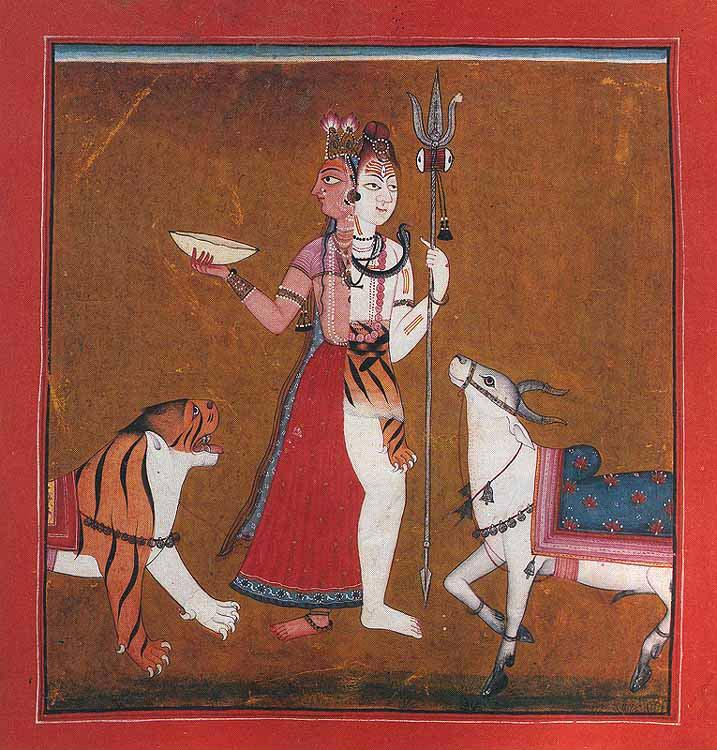
\includegraphics[width=0.7\textwidth]{androgyne.jpg}
    \end{center}
  \end{subfigure}
  \setcounter{figure}{1}
  \captionof{figure}{Śiva in their androgynous form of Ardhanārīśwara.}
  \label{siva}
\end{figure}

According to Serena Nanda,\footnote{Serena \cite{nanda} quotes Bullough pages 21–22.} Tantric Hinduism holds that all people contain both male and female principles within themselves. The Supreme Being is conceptualized as a complete hermaphrodite, which is the ideal. In some sects, males (never females) imitate women in dress and behavior to achieve salvation or to realize the `woman' in themselves in order to reach true love.

The other types of \textit{ubhatob­yañ­janakas} mentioned in the commentaries seem to be similar in their ability to have sex as both a male and a female, but being sterile in one of these faculties. Again, this is not something we naturally find in human beings but it is a theme extensively found in the Vedic myths.

The word \textit{ubhatob­yañ­janaka} does not appear in any texts outside of the Buddhist \textit{Vinaya} and the \textit{Vinaya} commentaries.\footnote{Appendix \ref{appendix2}, Figure \ref{sanskrit1} shows that the word \textit{ubhatob­yañ­janaka} does not appear in any Vedic or Brahmanical texts and only appears in the Buddhist texts.} It seems however logical that by the sheer definition of the \textit{napuṁsaka} as `anything that is not entirely male or female' the term \textit{ubhatob­yañ­janaka} also falls under this category. As a sub-category of the \textit{napuṁsaka} they would have been seen as hyperlibidinous, which is explained in later texts by the fact that \textit{napuṁsakas} have both male and female characteristics.\footnote{As we have seen in chapter \ref{linga} it is likely that `characteristics' are defined as more than merely genital or procreative. \cite{jackson}, quoting Bunmi Methangkun (1986) (article in Thai), observes that psychological as well as physiological factors are involved in the constitution of the \textit{ubhatob­yañ­janaka}. He also observes (without reference) that in early Buddhist communities men who engage in receptive anal sex are seen as feminized and thought to be hermaphrodites.} The explanation in the commentaries and sub-commentary as mentioned above also shows they are seen as bisexual in nature, similar to what we have seen in the Jain commentarial literature description of \textit{napuṁsaka}.

The term \textit{paṇḍaka} as a subset of \textit{napuṁsaka} was also seen as having both male and female characteristics in the Jain scriptures but is obviously not the same as the \textit{ubhatob­yañ­janaka}. The difference between the \textit{paṇḍaka} and the \textit{ubhatob­yañ­janaka} clearly seems to be on the procreative level in that the \textit{ubhatob­yañ­janaka} is able to conceive and impregnate while the \textit{paṇḍaka}, as an impotent man, can do neither. From the descriptions given in the \textit{Samantapāsādikā} we can also conclude that the \textit{ubhatob­yañ­janaka} is able to change their primary and secondary characteristics, including external appearance and behavior to appear to be either male or female. Again, this is not possible outside the realm of mythology.

All the \textit{Vinayas} agree that the \textit{ubhatob­yañ­janaka}/二根 is one of the four sex/gender types next to male, female and \textit{paṇḍaka}/黃門. Considering that males and females were both seen as having just one root/faculty (in the meaning of procreative ability), and the \textit{paṇḍaka} as having none,\footnote{Note that when the \textit{paṇḍaka} appears in the texts in the list of these four sex/gender types, it is always described in the Chinese \textit{Vinayas} with the characters 黃門 (`eunuch') and never as 不能男 (`impotent'). Indeed we find in the Chinese texts that a eunuch is somebody with the `male faculty' removed. There might be some confusion here as to what entails characteristics and the Chinese scribes would have only been able to describe this based on their own experiences in their own culture.} the person with two faculties fills a gap. Bee Scherer notes that this fourfold taxonomy (`male', `female', `both ...', `neither ...') is intended to achieve the Classical Indian (and especially Buddhist) fourfold logical tetralemma called the \textit{catuṣkoṭi}\footnote{\cite{scherer} page 68 and Dr. M. Vermeulen, whose book on this subject is yet to be published.} and that the categories of \textit{paṇḍaka} and \textit{ubhatob­yañ­janaka} are largely academic. This might indeed have played a role but I believe there are also other considerations like the fact that these types, either as mythological beings or the enactment thereof, are indeed found in India.

Just like the term \textit{paṇḍaka}, I believe that the \textit{ubhatob­yañ­janaka} is a later addition to the \textit{Vinaya}. The word only appears briefly in the \textit{Vinaya}. It does not appear in the early \textit{Suttas}, or in the \textit{Pāṭimokkhas}, or in other early parts of the \textit{Vinaya}.\footnote{See Appendix \ref{appendix2}, Figure \ref{pali1}.} The description is so brief and hardly existent in the Chinese texts that it seems to be added almost as an afterthought. Appendix \ref{appendix2}, Figure \ref{chinese1}, shows that the words used for the \textit{ubhatob­yañ­janaka} in the Chinese texts mainly appear in the \textit{Vinaya} collections T22–T24 and the later \textit{Abhidhamma} and commentaries as well as most prominently in T54, which are non-Buddhist texts. And again we see the same pattern in the Tibetan charts in Figure \ref{tibetan1}. The insertion of this word would have most likely occurred during the redaction of the \textit{Vinaya} at the Second Council as discussed in the previous chapter.

\textit{Ubhatob­yañ­janaka} seems to be a rather elusive term that does not allow itself to be captured easily. Various scholars have tried to explain this as a form of intersex\footnote{For a brief description of the term `intersex' see Appendix \ref{appendix3}, section \ref{intersex}.} for the sole reason that intersex people were previously erroneously called `hermaphrodite' and a hermaphrodite can procreate in both the male and female way as in the description of the \textit{ubhatob­yañ­janaka} in the commentaries. This is confusing as a true hermaphrodite does not exist among humans and is distinct from intersex. 

From the descriptions in the commentaries, the \textit{ubhatob­yañ­janaka} is not human in nature. It is a concept, a mythological being, the embodiment of the feminine principle in the male. And just like the \textit{paṇḍaka} it is likely that there were also people involved in the religious enactment of these mythological tales as we have seen in Tantric Hinduism, which would have included strong sexual motifs.\footnote{\cite{nanda} page 22.} It is likely that people with ambiguous genital characteristics were among these, as they naturally bear some resemblance to the idealized hermaphrodite Supreme Being, but the concept entailed more than just physical characteristics; it also involved gender-expression and social religious roles. As Robert \cite{goldman} points out: ``... the whole phenomenon appears to be deeply bound up with a patriarchal culture's ambivalent construction of women and their sexuality.'' The Vedic stories explore the deep longing of men to be able to conceive and this idea is found in a variety of Indian sources. Again, this is a concept that does not match any contemporary notions.
